\fancyhead[L]{Chapter II}
\fancyhead[R]{Analysis and Design}

\vspace*{9cm}
\begin{doublespace}
    \centering
    \addcontentsline{toc}{chapter}{Chapter II: Analysis and Design}
    \textbf{ \huge Chapter II \\ [1 cm] Analysis and Design}
\end{doublespace}

\newpage
\fancyhead[R]{\rightmark}

\setcounter{section}{0}
\section*{Introduction}

This chapter presents the analysis and design phase of the notification system for cryptographic resource management within the KMS. The analysis phase identifies the functional and non-functional requirements, while the design phase defines the system architecture, database structure, and component interactions necessary for implementing an automated audit and alert system for expirable cryptographic resources.

\section{Requirements Analysis}

\subsection{Functional Requirements}

The functional requirements describe the main features that the notification system must provide. Based on the analysis of the KMS context and user needs, the following functional requirements have been identified:

\subsubsection{Resource Discovery and Monitoring}

\textbf{Automatic Resource Detection:} The system must be capable of automatically discovering certificates and keys that are approaching their expiration date. This discovery process should scan the database daily to identify resources requiring notification.

\noindent
\textbf{Expiration Timeline Management:} The system must calculate the number of days remaining before each resource expires and maintain this information up-to-date to ensure accurate notification timing.

\noindent
\textbf{Resource Lifecycle Tracking:} The system must track the status of each resource throughout its lifecycle, from active use to expiration or renewal.

\subsubsection{Notification Management}

\textbf{Multi-Channel Communication:} The system must support multiple notification channels to ensure message delivery reliability:
\begin{itemize}
    \item Email notifications for formal communication
    \item In-app notifications for real-time alerts
    \item Configurable channel activation/deactivation
\end{itemize}

\noindent
\textbf{Role-Based Notification Targeting:} The system must identify and notify only relevant users based on their organizational roles:

\noindent
\textbf{Strategic Notification Scheduling:} The system must implement an intelligent notification schedule that provides timely alerts while minimizing notification fatigue. The timing should balance early warning with user experience.

\noindent
\textbf{Notification Status Management:} The system must track notification states throughout their lifecycle:
\begin{itemize}
    \item PENDING: notification created but not yet sent
    \item SENT: notification successfully delivered
    \item READ: user has acknowledged the notification
    \item FAILED: notification delivery failed
    \item CANCELLED: notification cancelled due to user response
    \item EXPIRED: resource has expired
    \item RENEWED: resource has been renewed
\end{itemize}

\subsubsection{User and Resource Management}

\textbf{Resource Response Tracking:} The system must allow users to mark resources as "responded to," automatically cancelling further notifications for those resources.

\noindent
\textbf{User Session Management:} For real-time notifications, the system must maintain active user sessions and route notifications to appropriate connected users.

\noindent
\textbf{Historical Tracking:} The system must maintain a complete audit trail of all notification activities for compliance and monitoring purposes.

\subsection{Non-Functional Requirements}

The non-functional requirements ensure the quality, performance, and reliability of the notification system:

\subsubsection{Performance Requirements}

\textbf{Scalability:} The system must handle a large number of users (hundreds) and resources (thousands) without performance degradation.

\noindent
\textbf{Concurrent Processing:} The system must support concurrent notification processing with configurable parallelism levels (2-5 concurrent email processing, 2-10 concurrent message processing).

\subsubsection{Reliability Requirements}

\textbf{Message Delivery Reliability:} The system must ensure reliable message delivery through:
\begin{itemize}
    \item Message queue persistence
    \item Automatic retry mechanisms with exponential backoff
    \item Dead letter queue handling for failed messages
    \item Message TTL configuration (10 minutes for email, 5 minutes for in-app)
\end{itemize}

\noindent
\textbf{Job Scheduling Reliability:} The system must ensure reliable execution of scheduled jobs:
\begin{itemize}
    \item Persistent job storage
    \item Automatic job recovery after system restart
    \item Job execution monitoring and logging
\end{itemize}

\newpage
\section{System Analysis}

\subsection{Use Case Analysis}

The use case analysis identifies the main actors and their interactions with the notification system.

\subsubsection{Main Use Cases}

% TODO: Insert Use Case Diagram here
\begin{figure}[H]
    \centering
    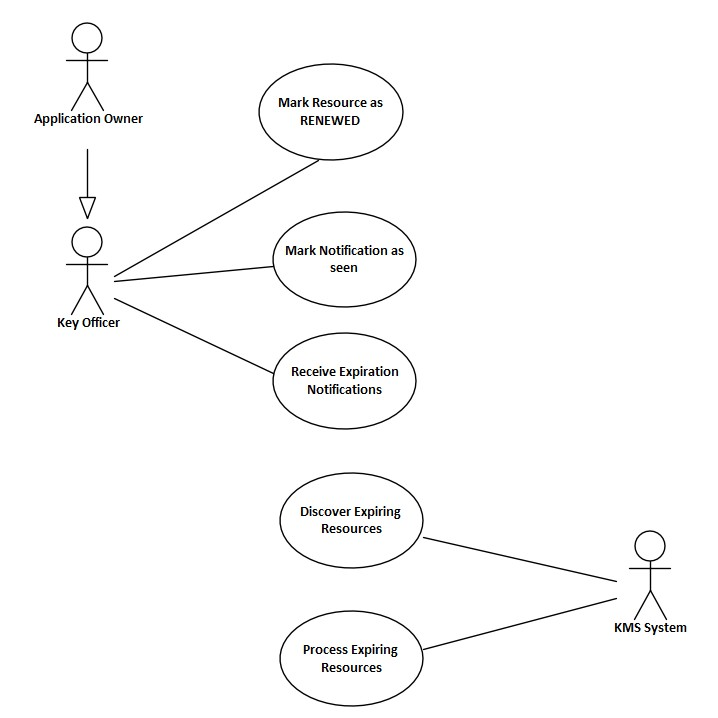
\includegraphics[width=0.8\textwidth]{images/use_case_diagram.jpg}
    \caption{Use Case Diagram - Notification System}
    \label{fig:use_case_diagram}
\end{figure}

\textbf{UC1: Receive Expiration Notifications}
\begin{itemize}
    \item \textbf{Actor:} Application Owner, Key Officer
    \item \textbf{Description:} Users receive notifications about expiring resources through email and in-app channels
    \item \textbf{Preconditions:} User has appropriate role assignment for the resource
    \item \textbf{Main Flow:} 
        \begin{enumerate}
            \item System discovers expiring resource
            \item System identifies responsible users
            \item System sends notifications via configured channels
            \item User receives and acknowledges notification
        \end{enumerate}
\end{itemize}

\noindent
\textbf{UC2: Mark Resource as Renewed}
\begin{itemize}
    \item \textbf{Actor:} Application Owner, Key Officer
    \item \textbf{Description:} Users indicate they have renewed an expiring resource
    \item \textbf{Preconditions:} User has received notification for the resource
    \item \textbf{Main Flow:}
        \begin{enumerate}
            \item User accesses notification system
            \item User selects resource to mark as renewed
            \item System cancels future notifications for the resource
            \item System updates resource status to RENEWED
        \end{enumerate}
\end{itemize}

\section{System Design}

\subsection{System Architecture}

The notification system follows a layered architecture pattern that ensures separation of concerns and maintainability.

\subsubsection{Architectural Overview}

% TODO: Insert System Architecture Diagram
\begin{figure}[H]
    \centering
    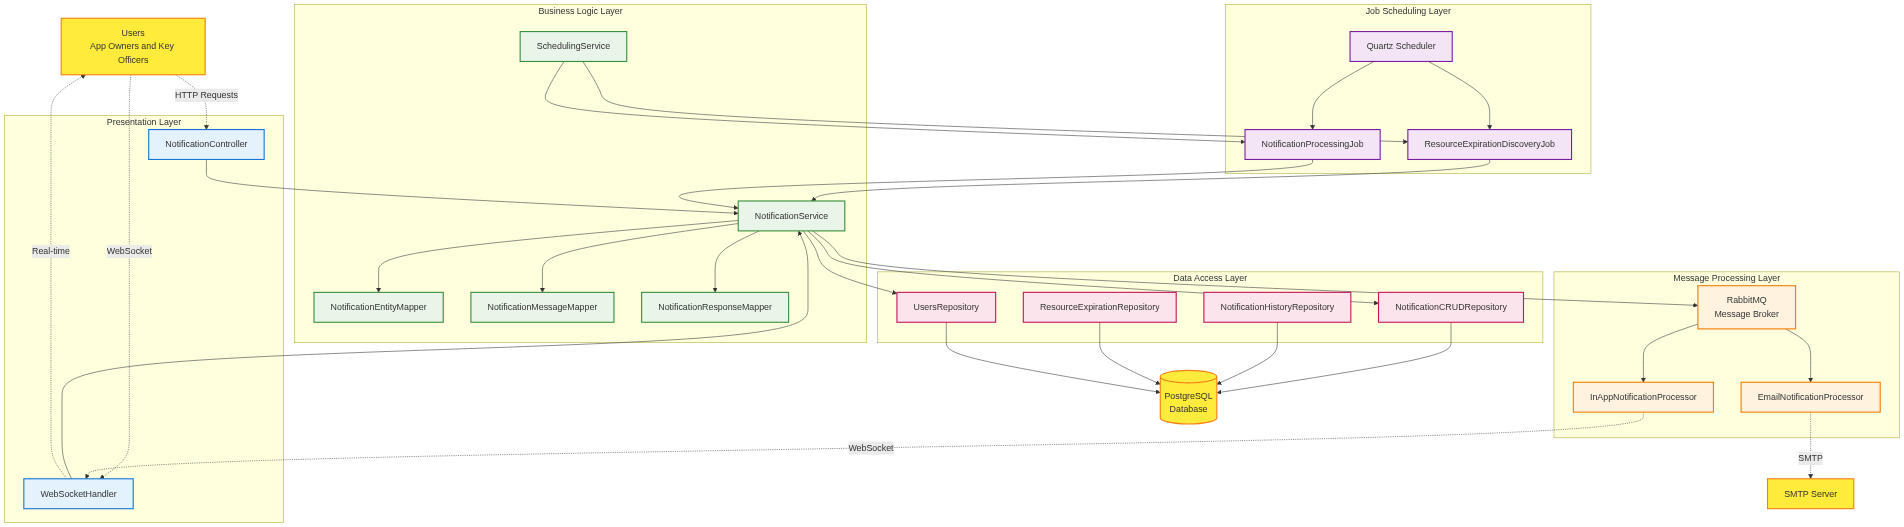
\includegraphics[width=1\textwidth]{images/system_architecture.png}
    \caption{System Architecture Overview}
    \label{fig:system_architecture}
\end{figure}

\textbf{Presentation Layer:}
\begin{itemize}
    \item \textbf{REST Controllers:} Handle HTTP requests and responses
        \begin{itemize}
            \item NotificationController: manages notification operations
            \item ManualSchedulingController: provides administrative functions
        \end{itemize}
    \item \textbf{WebSocket Handlers:} Manage real-time communication
        \begin{itemize}
            \item NotificationWebSocketHandler: handles in-app notifications
        \end{itemize}
\end{itemize}

\noindent
\textbf{Business Logic Layer:}
\begin{itemize}
    \item \textbf{Service Classes:} Implement core business logic
        \begin{itemize}
            \item NotificationService: manages notification lifecycle
            \item SchedulingService: handles manual job execution
        \end{itemize}
    \item \textbf{Mapper Classes:} Handle object transformations
\end{itemize}

\noindent
\textbf{Data Access Layer:}
\begin{itemize}
    \item \textbf{JPA Repositories:} Provide data persistence operations
        \begin{itemize}
            \item NotificationCRUDRepository: CRUD operations for notifications
            \item NotificationHistoryRepository: audit trail management
            \item ResourceExpirationRepository: resource discovery queries
        \end{itemize}
\end{itemize}

\noindent
\textbf{Message Processing Layer:}
\begin{itemize}
    \item \textbf{Message Processors:} Handle asynchronous notification delivery
        \begin{itemize}
            \item EmailNotificationProcessor: processes email notifications
            \item InAppNotificationProcessor: processes in-app notifications
        \end{itemize}
    \item \textbf{Message Queue:} RabbitMQ for reliable message delivery
\end{itemize}

\noindent
\textbf{Job Scheduling Layer:}
\begin{itemize}
    \item \textbf{Quartz Jobs:} Automated background processing
        \begin{itemize}
            \item ResourceExpirationDiscoveryJob: discovers expiring resources
            \item NotificationProcessingJob: processes scheduled notifications
        \end{itemize}
\end{itemize}

\subsection{Database Design}

\subsubsection{Database Schema}

The notification system extends the existing KMS database with two new entities designed to manage the complete lifecycle of expiration notifications.

\noindent
\textbf{Notification Entity:}
The primary entity that stores notification records with the following key attributes:

\noindent
\textbf{NotificationHistory Entity:}
An audit entity that preserves snapshots of notification state at the time of sending:

\noindent
These entities integrate seamlessly with existing KMS tables through foreign key relationships while maintaining data consistency and referential integrity.

\begin{figure}[H]
    \centering
    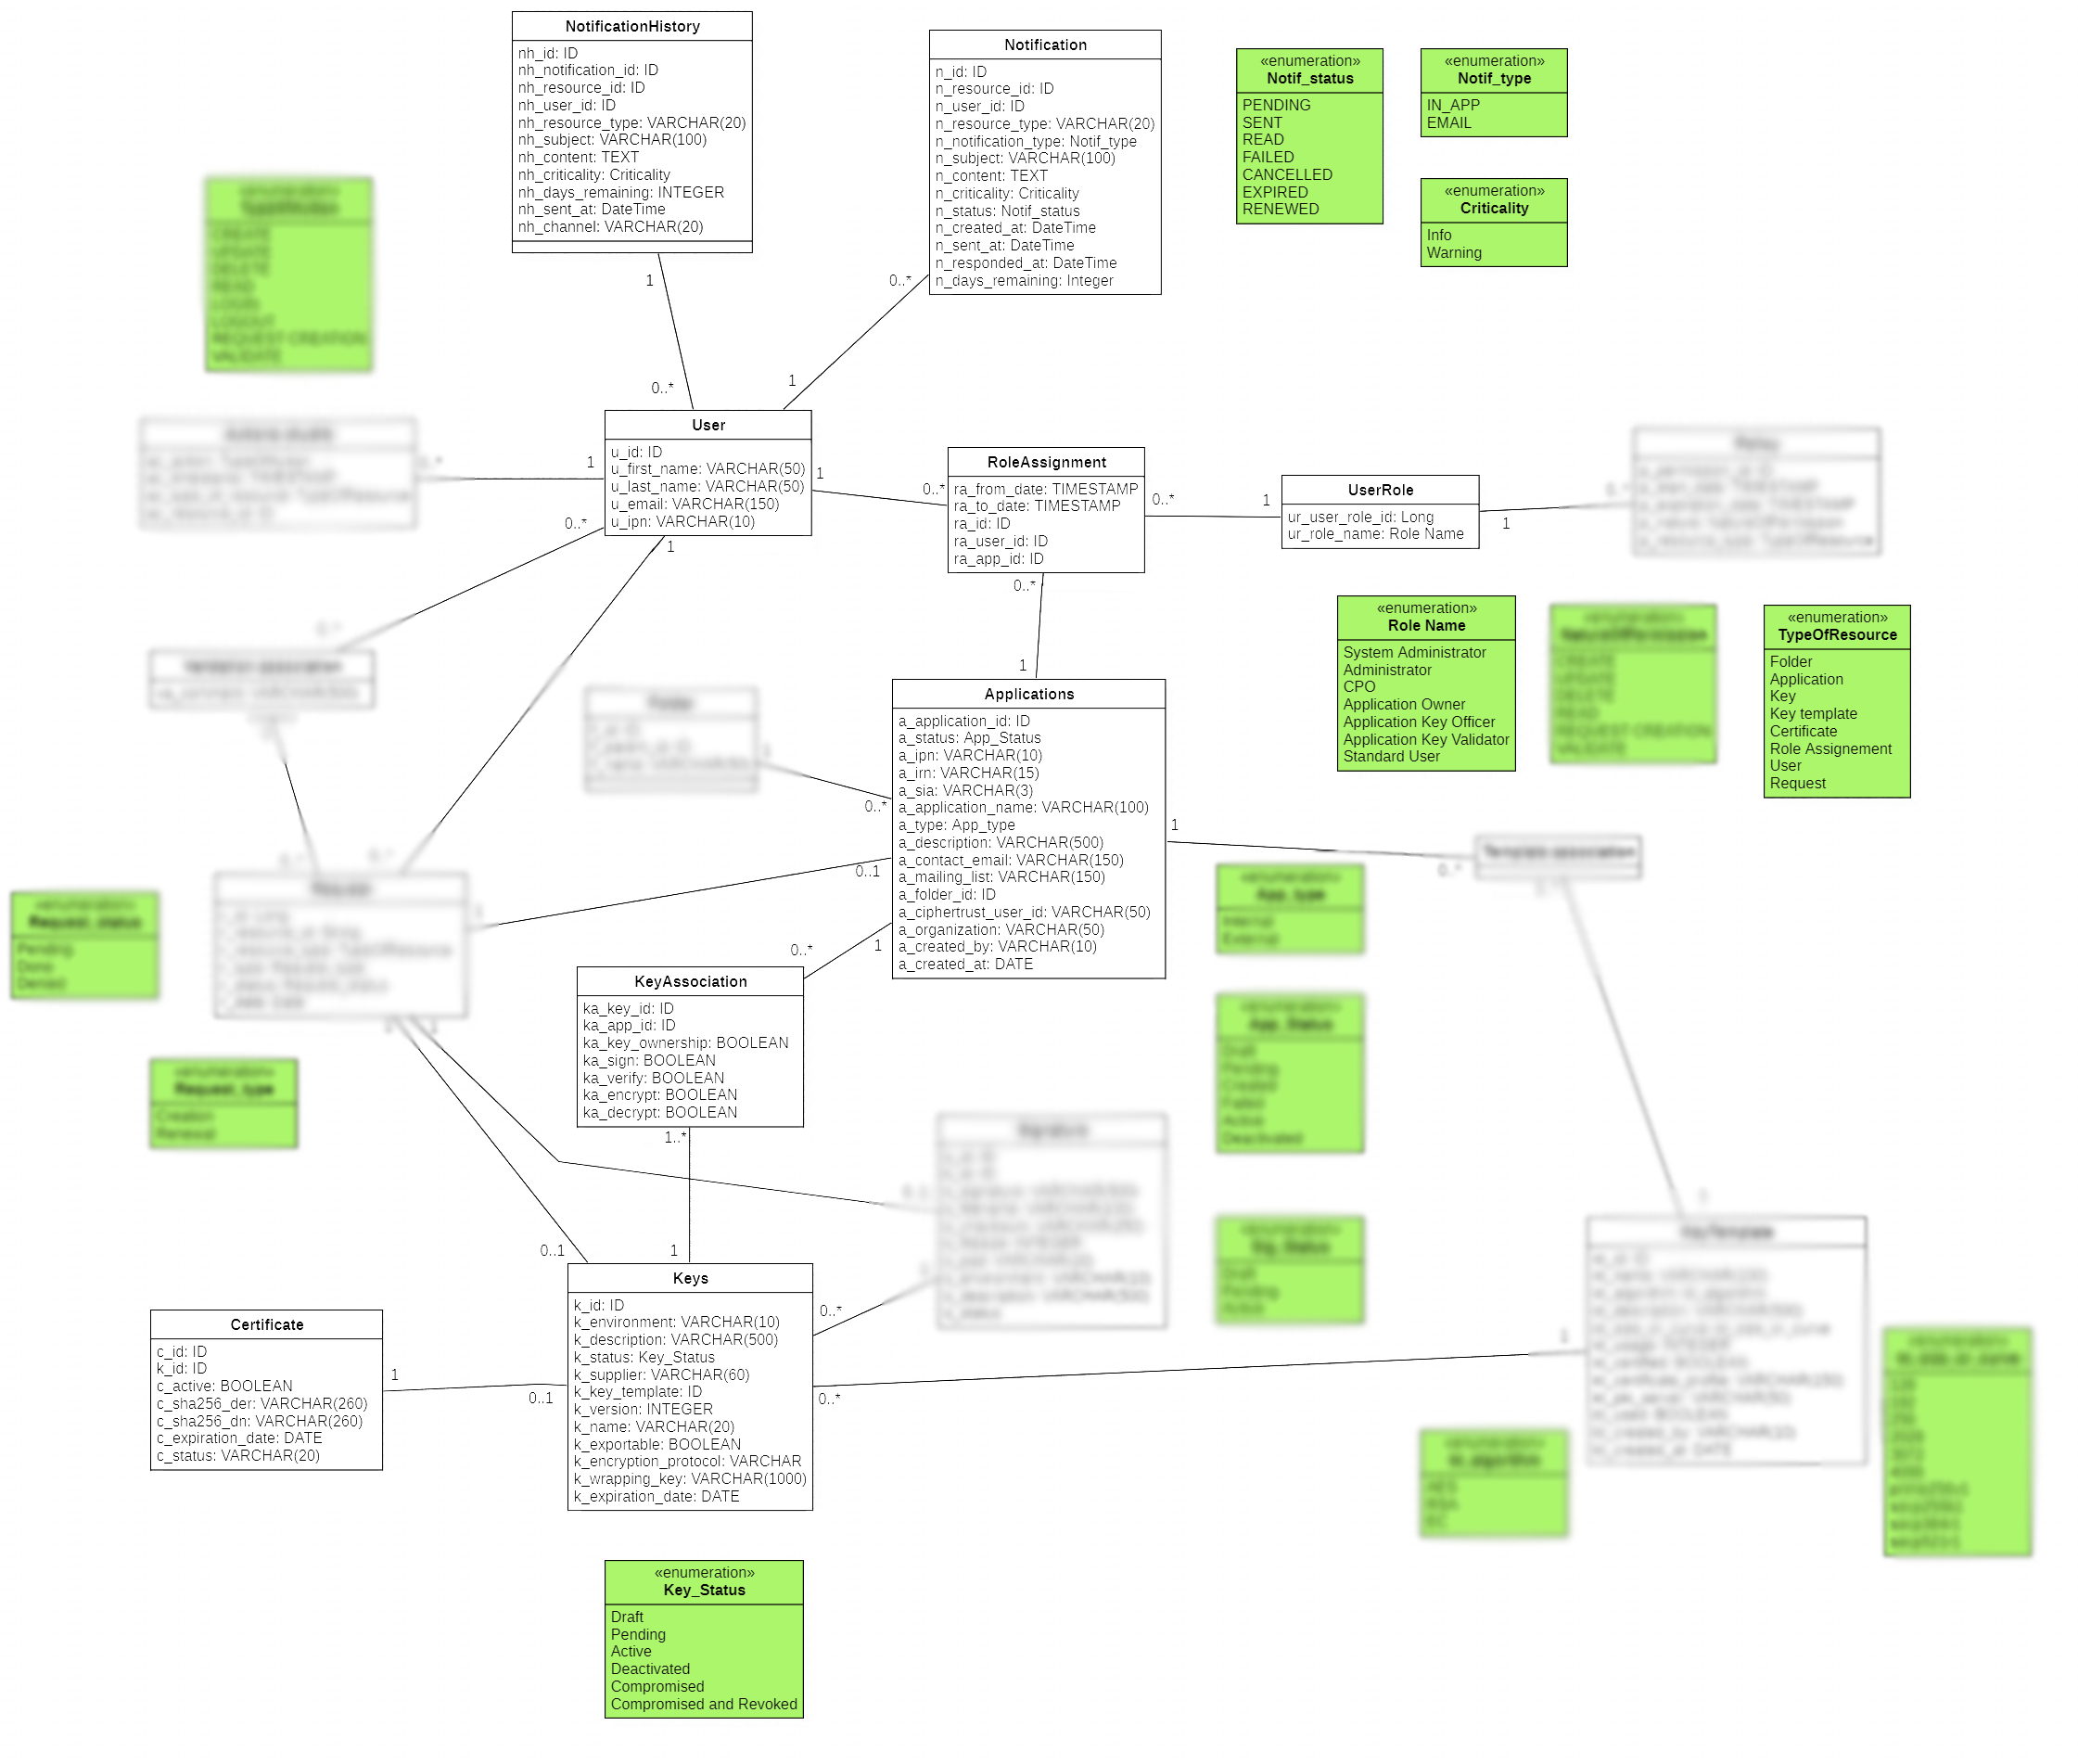
\includegraphics[width=1\textwidth]{images/database_schema.png}
    \caption{Database Schema}
    \label{fig:database_schema}
\end{figure}

\subsection{Component Design}

\subsubsection{Resource Discovery and Notification Processing}

The notification system operates through two distinct but interconnected processes: resource discovery and notification processing. These processes are implemented as separate Quartz jobs to ensure optimal performance and clear separation of concerns.

\newpage
\noindent
\textbf{Resource Discovery Process:}

% TODO: Insert Resource Discovery Diagram
\begin{figure}[H]
    \centering
    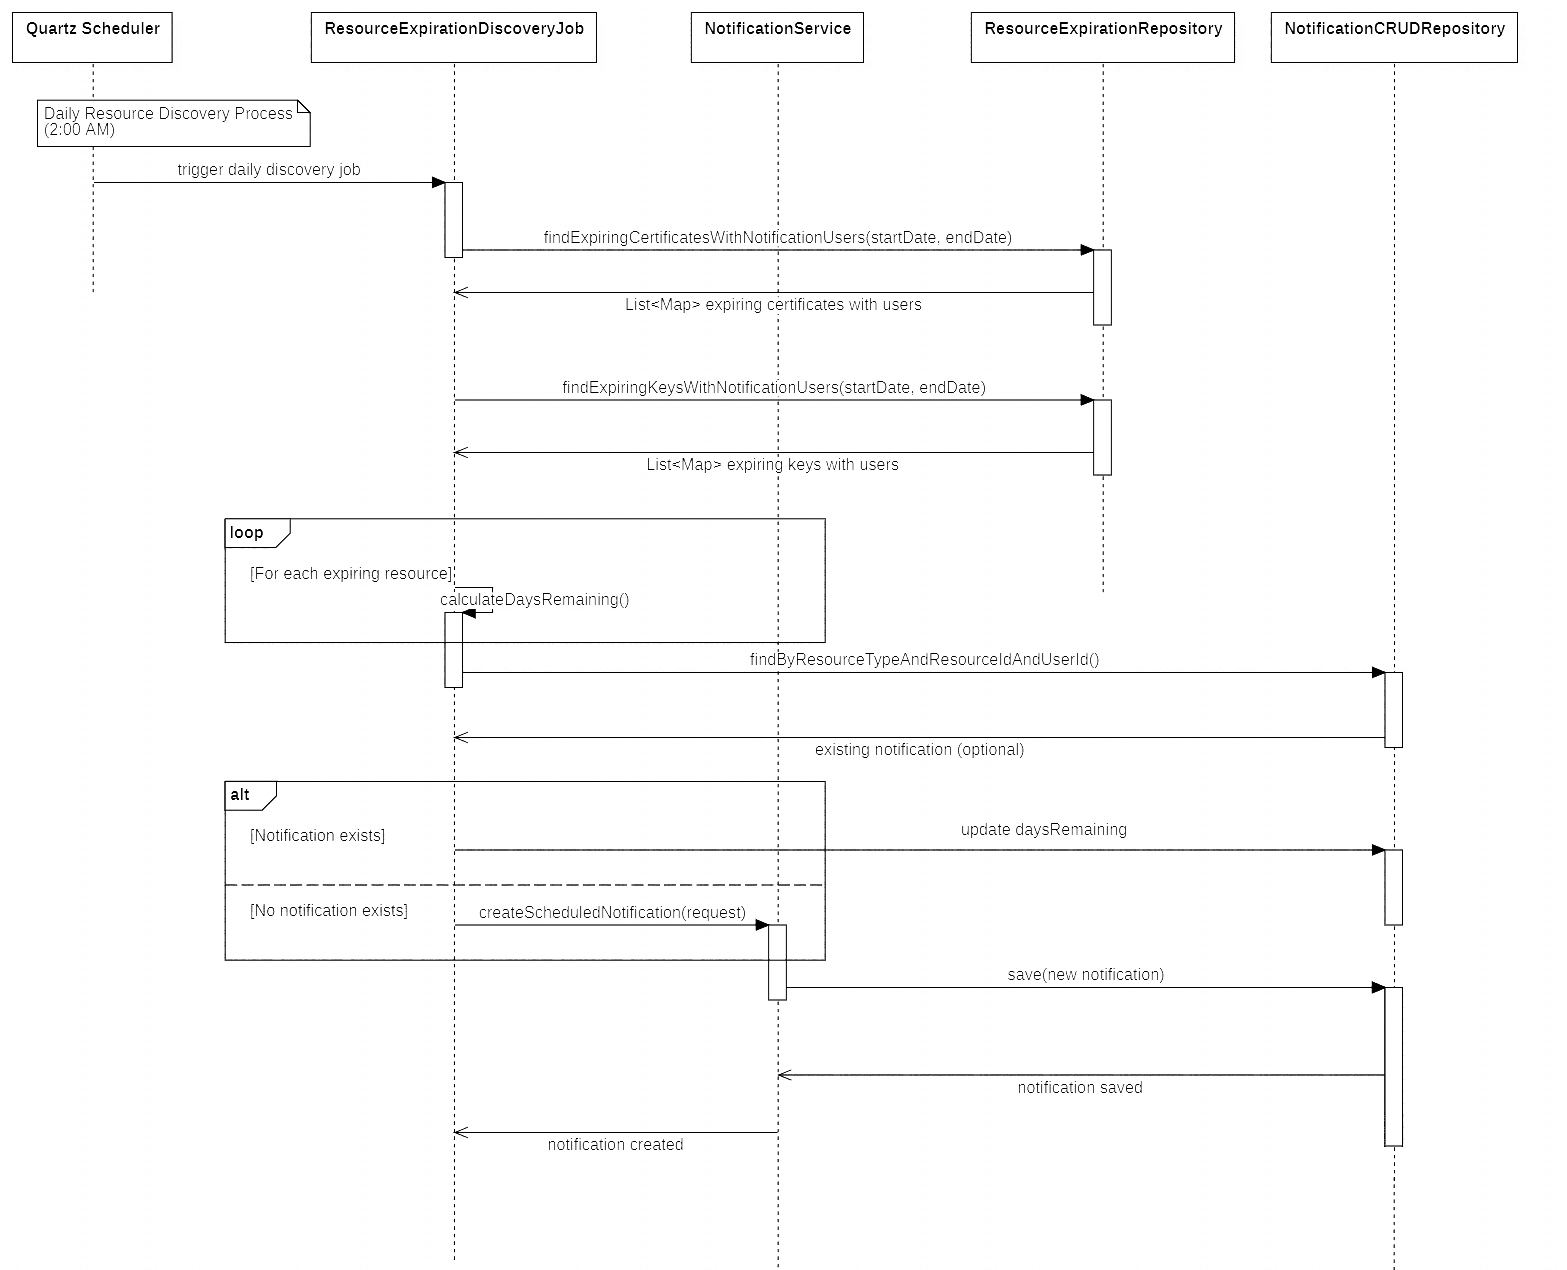
\includegraphics[width=1\textwidth]{images/resource_discovery_sequence.png}
    \caption{Resource Discovery Sequence Diagram}
    \label{fig:resource_discovery_sequence}
\end{figure}

\noindent
The ResourceExpirationDiscoveryJob executes daily at 2:00 AM to identify expiring cryptographic resources. The process queries both certificates and keys approaching expiration, identifies responsible users based on their role assignments, and creates or updates notification records. For existing notifications, the system updates the days remaining and resource status, while new expiring resources trigger the creation of scheduled notification records.

\newpage
\noindent
\textbf{Notification Processing and Delivery:}

% TODO: Insert Notification Processing Diagram
\begin{figure}[H]
    \centering
    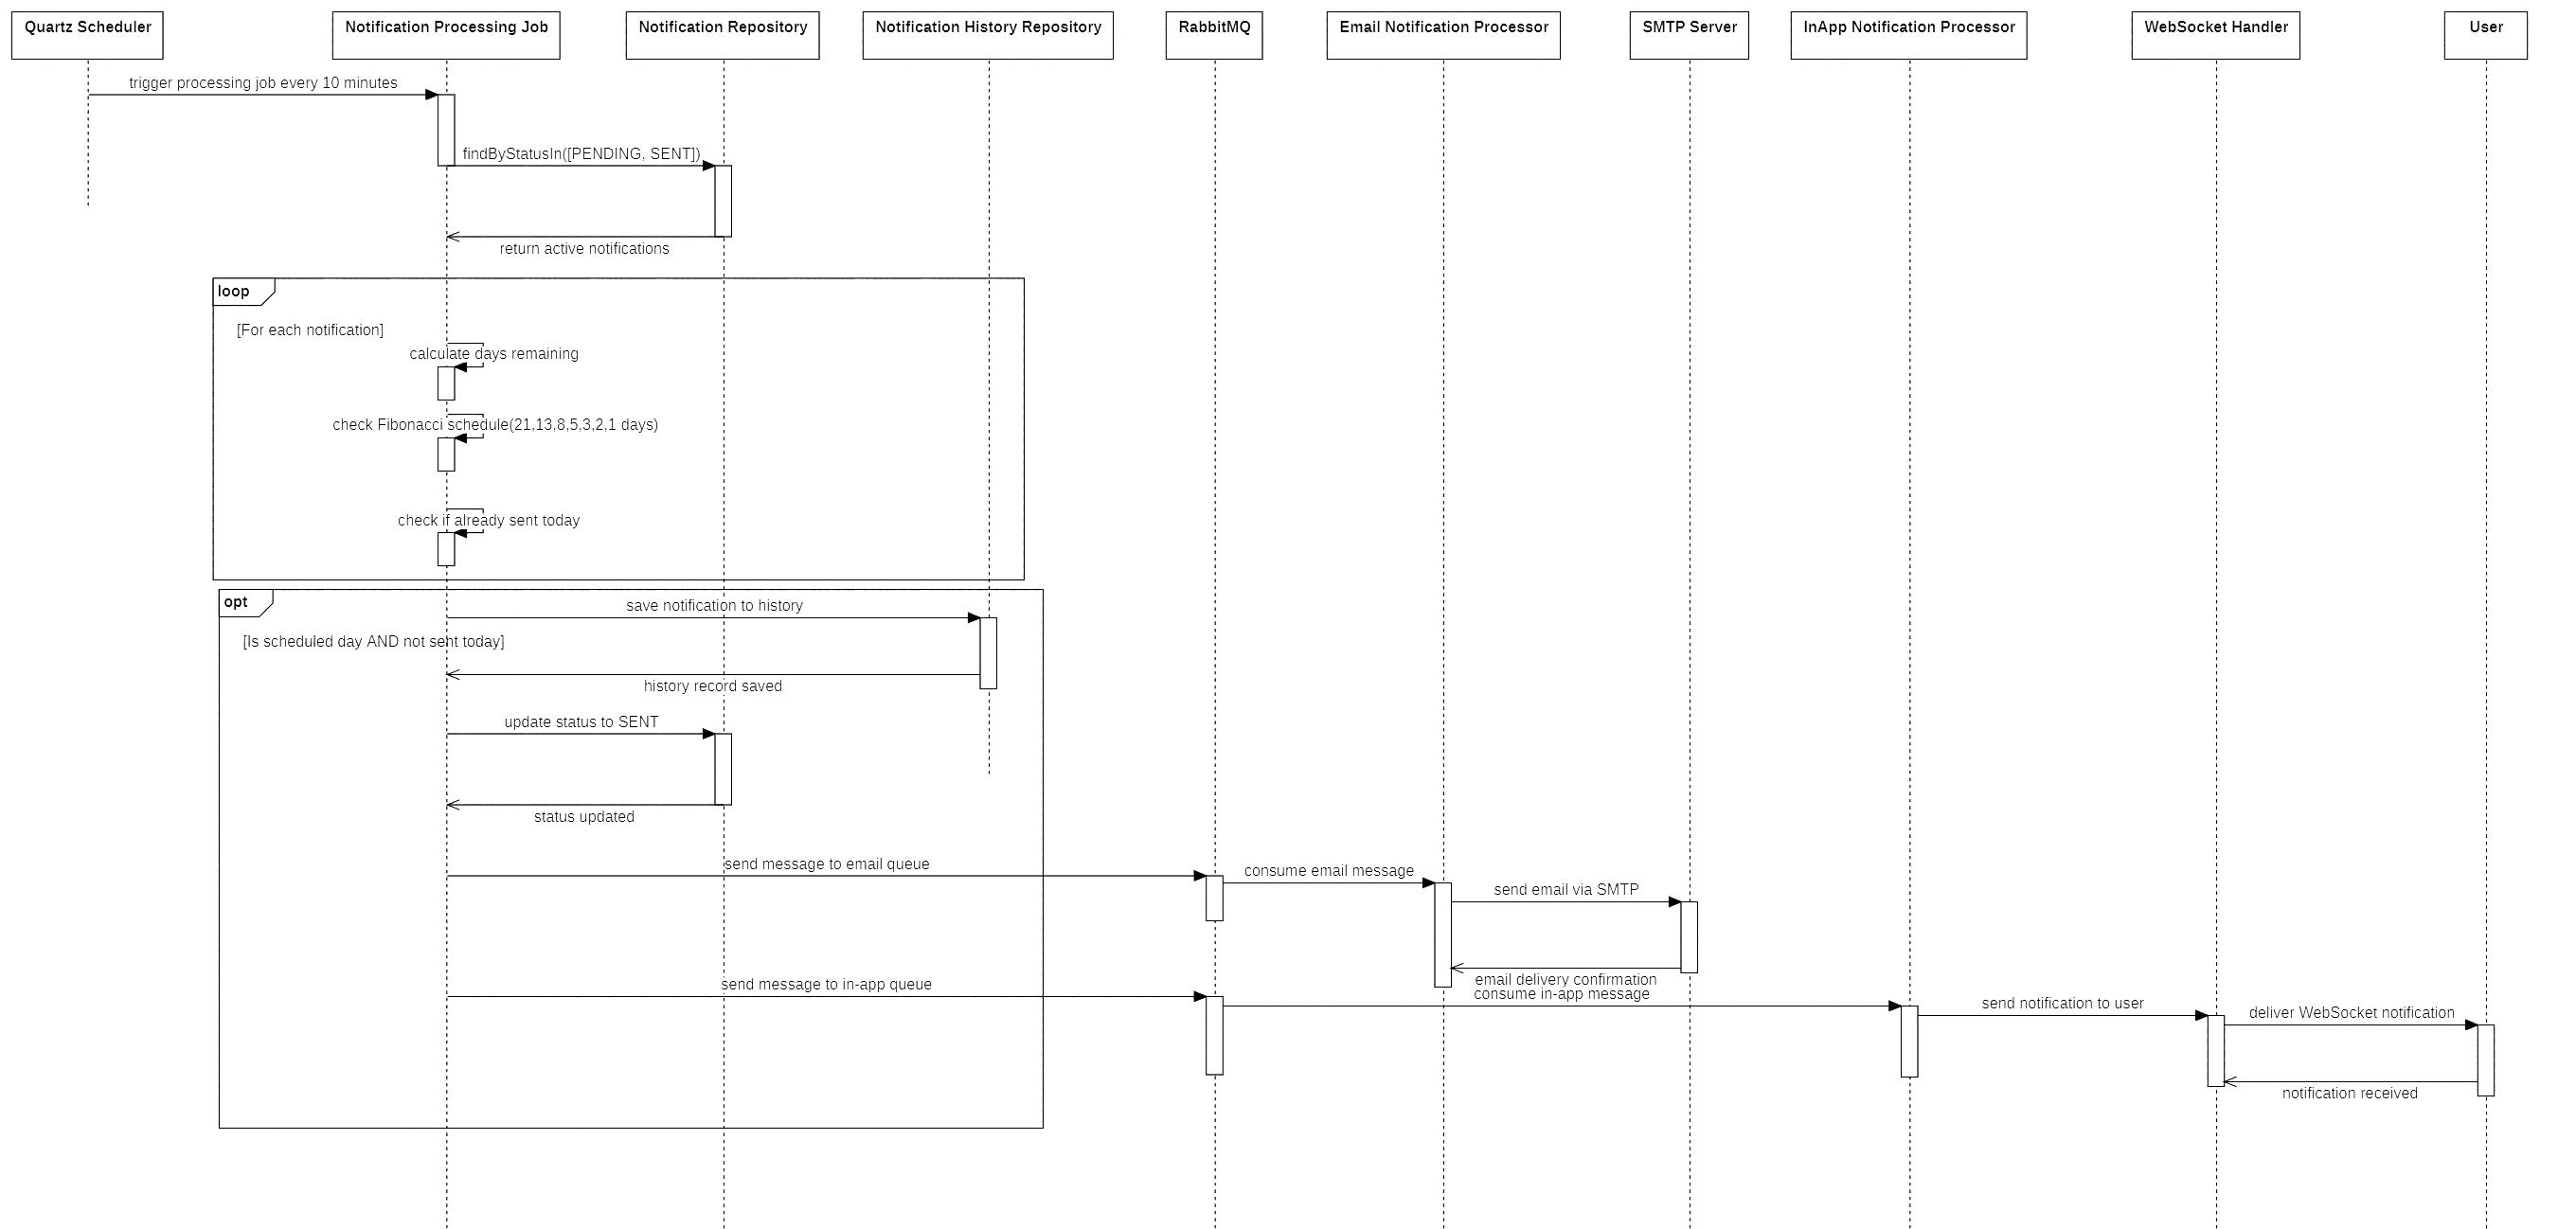
\includegraphics[width=1\textwidth]{images/notification_processing_sequence.png}
    \caption{Notification Processing and Delivery Sequence Diagram}
    \label{fig:notification_processing_sequence}
\end{figure}

\noindent
The NotificationProcessingJob executes every 10 minutes to process pending notifications using the Fibonacci scheduling algorithm (21, 13, 8, 5, 3, 2, 1 days before expiration). For notifications scheduled to be sent, the system saves a historical record, updates the notification status, and queues messages for both email and in-app delivery. The parallel processing architecture ensures that email notifications are sent via SMTP while in-app notifications are delivered through WebSocket connections, providing users with immediate awareness through multiple channels.\\

\noindent
\textbf{Scheduling Strategy:}

\noindent
The Fibonacci sequence provides an optimal balance between early warning and notification frequency. Users receive their first notification 21 days before expiration, with subsequent reminders following the mathematical sequence, creating increased urgency as the expiration date approaches while avoiding notification fatigue during the early warning period.

\newpage
\subsubsection{Message Queue Design}

% TODO: Insert RabbitMQ Architecture Diagram
\begin{figure}[H]
    \centering
    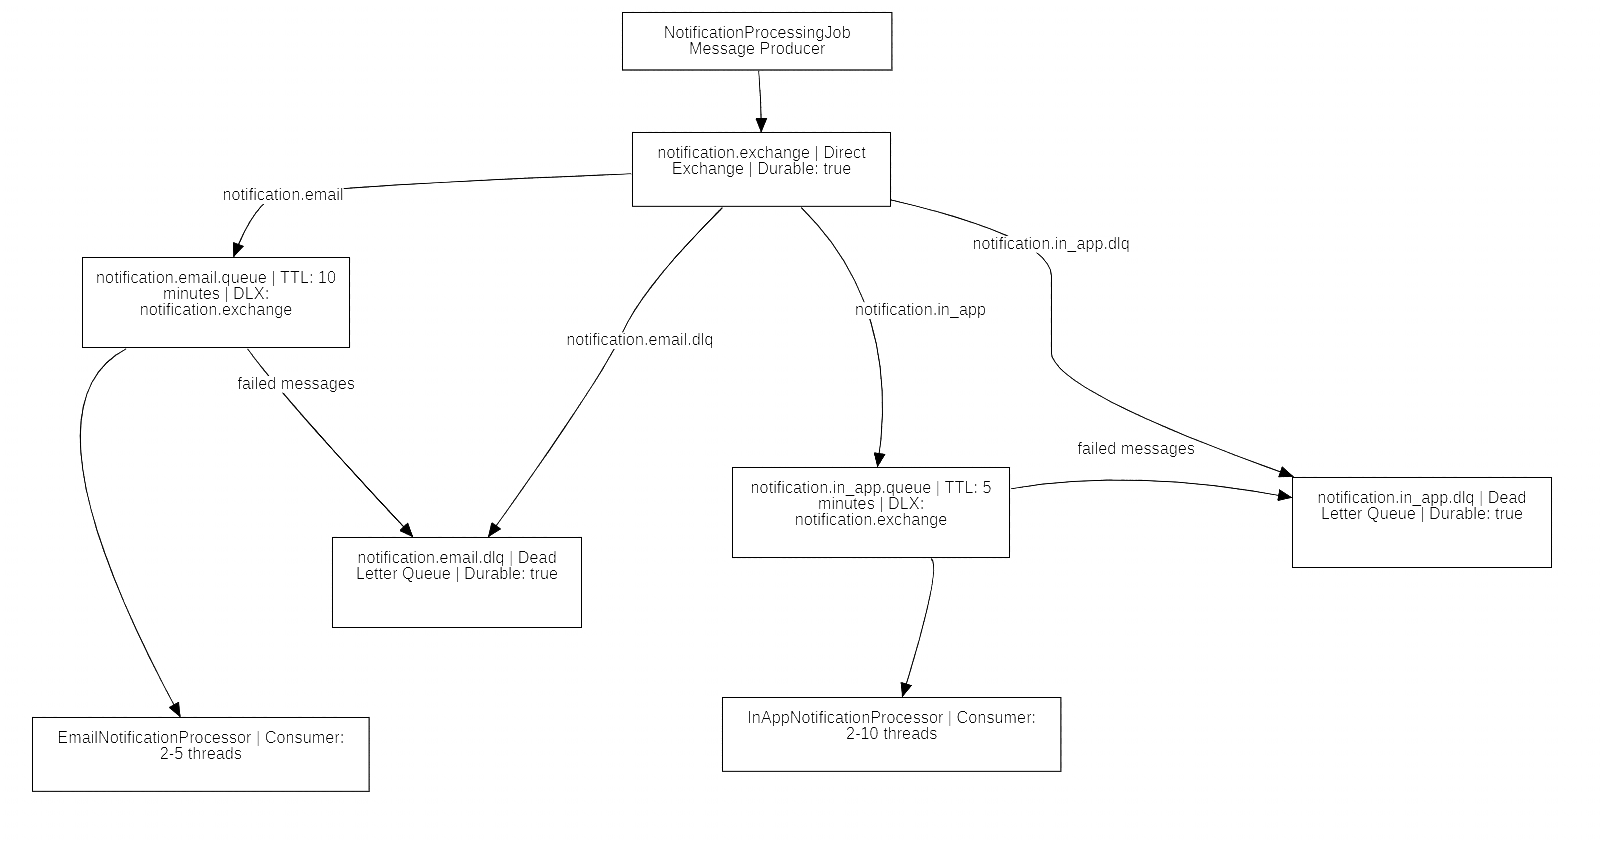
\includegraphics[width=1\textwidth]{images/rabbitmq_architecture.png}
    \caption{RabbitMQ Message Queue Architecture}
    \label{fig:rabbitmq_architecture}
\end{figure}

\textbf{Message Queue Architecture Design:}

\noindent
The notification system employs RabbitMQ as a message broker to ensure reliable and scalable message delivery through a carefully designed architecture. The system utilizes a \textbf{direct exchange} (notification.exchange), which routes messages to queues based on exact routing key matches, providing precise control over message distribution. When the NotificationProcessingJob publishes a message with routing key "notification.email", the direct exchange routes it exclusively to the email queue, while messages with "notification.in\_app" routing keys are directed to the in-app notification queue. This routing mechanism ensures clean separation between notification channels and prevents message misdelivery.

\noindent
To enhance system reliability, the architecture implements \textbf{dead letter queues} (DLQ) as a failure recovery mechanism. When messages in the primary queues exceed their time-to-live (TTL) limits or fail processing after maximum retry attempts, they are automatically redirected to their respective dead letter queues rather than being permanently lost. Email notifications have a 10-minute TTL to accommodate potential SMTP server delays, while in-app notifications use a shorter 5-minute TTL due to their real-time nature. The dead letter queues preserve failed messages for manual inspection and reprocessing, ensuring that critical expiration notifications are never permanently lost due to temporary system issues. This design provides both operational resilience and comprehensive audit capabilities, essential for maintaining the integrity of the cryptographic resource lifecycle management system.


\section*{Conclusion}

This chapter established the analytical foundation and design framework for the notification system within the KMS architecture. The requirements analysis identified the need for automated resource discovery, intelligent notification scheduling, and multi-channel communication to manage cryptographic resource lifecycles effectively.

\noindent
The system design presented a layered architecture promoting separation of concerns through distinct presentation, business logic, data access, message processing, and job scheduling layers. The database design integrates two new entities—Notification and NotificationHistory—with the existing KMS schema while enabling comprehensive audit capabilities. The component design detailed the workflow involving resource discovery jobs, Fibonacci-based scheduling algorithms, and parallel message processing through RabbitMQ infrastructure.

\noindent
This design foundation provides the blueprint for implementing an intelligent notification system that proactively manages cryptographic resource expirations, reducing operational risk and enhancing security compliance. The following chapter will detail the actual implementation of these design specifications.